%%%%%%%%%%%%%%%%%%%%%%%%%%%%%%%%%%%%%%%%%%%%%%%%%%%%%%%%%%%%%%%%%%%%%%
% LaTeX Example: Project Report
%
% Source: http://www.howtotex.com
%
% Feel free to distribute this example, but please keep the referral
% to howtotex.com
% Date: March 2011
%
% Edit the title below to update the display in My Documents
%\title{Project Report}
%
%%% Preamble
\documentclass[paper=a4, fontsize=11pt]{scrartcl}
\usepackage[T1]{fontenc}
\usepackage{fourier}

\usepackage[english]{babel}  % English language/hyphenation
\usepackage[protrusion=true,expansion=true]{microtype}
\usepackage{amsmath,amsfonts,amsthm} % Math packages
\usepackage[pdftex]{graphicx}
\usepackage{url}


%%% Custom sectioning
\usepackage{sectsty}
%\allsectionsfont{\centering \normalfont\scshape}   %original
\allsectionsfont{\normalfont\scshape}

%%% By Davide
\usepackage{comment}
\usepackage{float}
\floatstyle{boxed}
\newfloat{fragment}{htb}{fragment}
\floatname{fragment}{Fragment}

\usepackage{framed}
\usepackage{fancyvrb}
\RecustomVerbatimEnvironment{Verbatim}{Verbatim}{fontsize=\footnotesize,baselinestretch=.9}
\usepackage{listings}

\usepackage[export]{adjustbox}

\usepackage{courier}
%\newcommand{\mono}[1]{\texttt{\textbf{#1}}}
\newcommand{\mono}[1]{\texttt{#1}}

\usepackage[square,numbers]{natbib} % customize citation style
\usepackage[hidelinks]{hyperref}  % \href and \url tags, clickable crossref
\usepackage{subcaption}

\usepackage[section,nottoc]{tocbibind}
\renewcommand\tocbibname{\refname}  % tocbibind will use "References" rather than "Bibliography"

%%% Custom headers/footers (fancyhdr package)
\usepackage{fancyhdr}
\pagestyle{fancyplain}
\fancyhead{}                                            % No page header
\fancyfoot[L]{Davide Kirchner}
\fancyfoot[C]{Scheduletrace}
\fancyfoot[R]{\thepage}                                 % Pagenumbering
\renewcommand{\headrulewidth}{0pt}          % Remove header underlines
\renewcommand{\footrulewidth}{0pt}              % Remove footer underlines
\setlength{\headheight}{13.6pt}


%%% Equation and float numbering
\numberwithin{equation}{section}        % Equationnumbering: section.eq#
\numberwithin{figure}{section}          % Figurenumbering: section.fig#
\numberwithin{table}{section}               % Tablenumbering: section.tab#
\numberwithin{fragment}{section}


%%% Maketitle metadata
\newcommand{\horrule}[1]{\rule{\linewidth}{#1}}     % Horizontal rule

\title{
        \vspace{-1in}
        \usefont{OT1}{bch}{b}{n}
        \normalfont \normalsize \textsc{Graduate Program in Computer Science and Engineering} \\
        \normalfont \normalsize \textsc{DISI, University of Trento | TeCIP, Scuola Sant'Anna, Pisa} \\ [6pt]
        \normalfont \normalsize \textsc{Real-Time Systems: course project} \\ [25pt]
        \horrule{0.5pt} \\[0.4cm]
        \huge Scheduletrace: a schedule visualizer for Linux \\
        \horrule{2pt} \\[0.5cm]
}
\author{
        \normalfont                                 \normalsize
        Author: Davide Kirchner \\[-3pt]  \normalsize
        
\includegraphics[height=1.8ex]{img/addr.png}\vspace{-.4ex}\\[-3pt]     \normalsize
        Student ID 167679 (UniTN) \\[-3pt]     \normalsize
        Supervisor: prof. Giorgio Buttazzo \\[-3pt]      \normalsize
        %[DRAFT]
        \today
}
\date{}

% Words that flyspell should not mark red: Trento Davide Kirchner behaviour behaviours struct taskset

%%% Begin document
\begin{document}
\maketitle

\setcounter{tocdepth}{3}
\tableofcontents
\clearpage

\section{Introduction}\label{sec:intro}
This document describes \mono{scheduletrace}, a utility to graphically display the scheduling of a set of ad-hoc periodic tasks running on a Linux system.

Section~\ref{sec:usage} provides an introduction to the program's features and its usage. Section~\ref{sec:arch} describes the program's architecture, detailing its main components and digging into some of the implementation issues that arose during its development. Section~\ref{sec:runs} shows the outcome of running a priority-inversion--prone task set with the three different available priority-inversion protocols.


\section{Usage}\label{sec:usage}
The user interface articulates into two main types of interactions: command-line parameters that affect the behaviour of the program and shall be specified when launching the application, and the interactive commands needed to control the task set and its visualization on the fly.

\subsection{Command-line arguments}
Most of the command-line arguments deal with controlling the inputs and outputs of the program, ranging from controlling the logging verbosity (\mono{-q}, \mono{-v}) to the size of the graphical window (\mono{-H} and \mono{-W}). Most notably, the \mono{-f FILE} argument can be used to read the task set specification from a file (defaulting to the standard input), with the syntax described in the README file: a task is described by its period, relative deadline, priority and by a list of instructions of the type ``run \textit{x} operations while owning resource R\textit{n}''.

Other interesting command-line parameters are detailed in section~\ref{sec:arch} when appropriate, while the complete list of valid arguments can be obtained by running the program with the \mono{-h} or \mono{-{}-help} flag.

\subsection{Interactive commands}

\begin{figure}
  \centering
  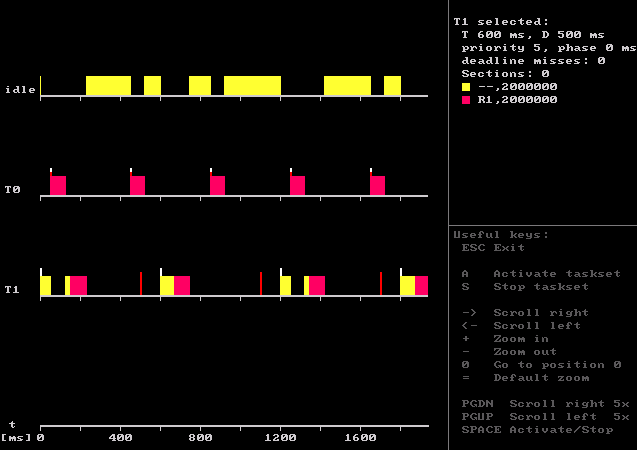
\includegraphics[width=.85\textwidth,frame]{img/gui.png}
  \caption{\label{fig:gui} The graphical user interface during a sample run.}
\end{figure}

When running with the Graphical user interface, the user is presented with a screen divided into three sections: the biggest one on the left is dedicated for the display of scheduling information, while the rightmost section is further split into two, for displaying contextual information and for providing the list of available commands.

After the GUI has loaded, the user can issue the following commands:
\begin{itemize}
\item \textit{A}: Activate the task set.
\item \textit{S}: Stop the task set.
\item \textit{Space}: Behaves as either \textit{A} or \textit{S}, according to the situation.
\item \textit{+}/\textit{-}: Adjust the scale on the time axis.
\item \textit{P}/\textit{M}: Aliases for \textit{+}/\textit{-}, more comfortable but less intuitive.
\item \textit{=}: Restore the default zoom level.
\item $\leftarrow$/$\rightarrow$: Pan the time axis to the left or right. The shift amount depends on the current zoom level, so as to result in a comparable on-screen distance regardless of the zoom level.
\item \textit{PgUp}/\textit{PgDown}: Pan the time axis 5 times faster than the corresponding arrows.
\item \textit{0}: Pan the time axis to position 0.
\item $\uparrow$/$\downarrow$: Select a previous/next task, respectively.
\item \textit{Q}, \textit{Esc} or \textit{Control-C}: Instruct the program to exit gracefully, terminating the task set if still active.
\item \textit{R} or \textit{F5}: Forces the GUI to redraw itself. Although this should never be needed in practice, it has been added for debugging purposes, and might turn useful in case of any GUI-related malfunctioning.
\end{itemize}

Note that it is not possible to restart a stopped task set while keeping the same trace. The task set can simply be restarted by quitting and re-running the application.


\section{Architecture}\label{sec:arch}

At the program start-up, the taskset file is parsed: for each periodic task a \mono{struct task} is initialized. In the meanwhile, the shared resources (i.e. instances of \mono{struct resource\_set}) required by the task set are initialized, and finally one thread per task is created. After creation, each thread waits on its activation semaphore until the user instructs the activation, which happens synchronously for all the tasks.

\begin{figure}
  \centering
  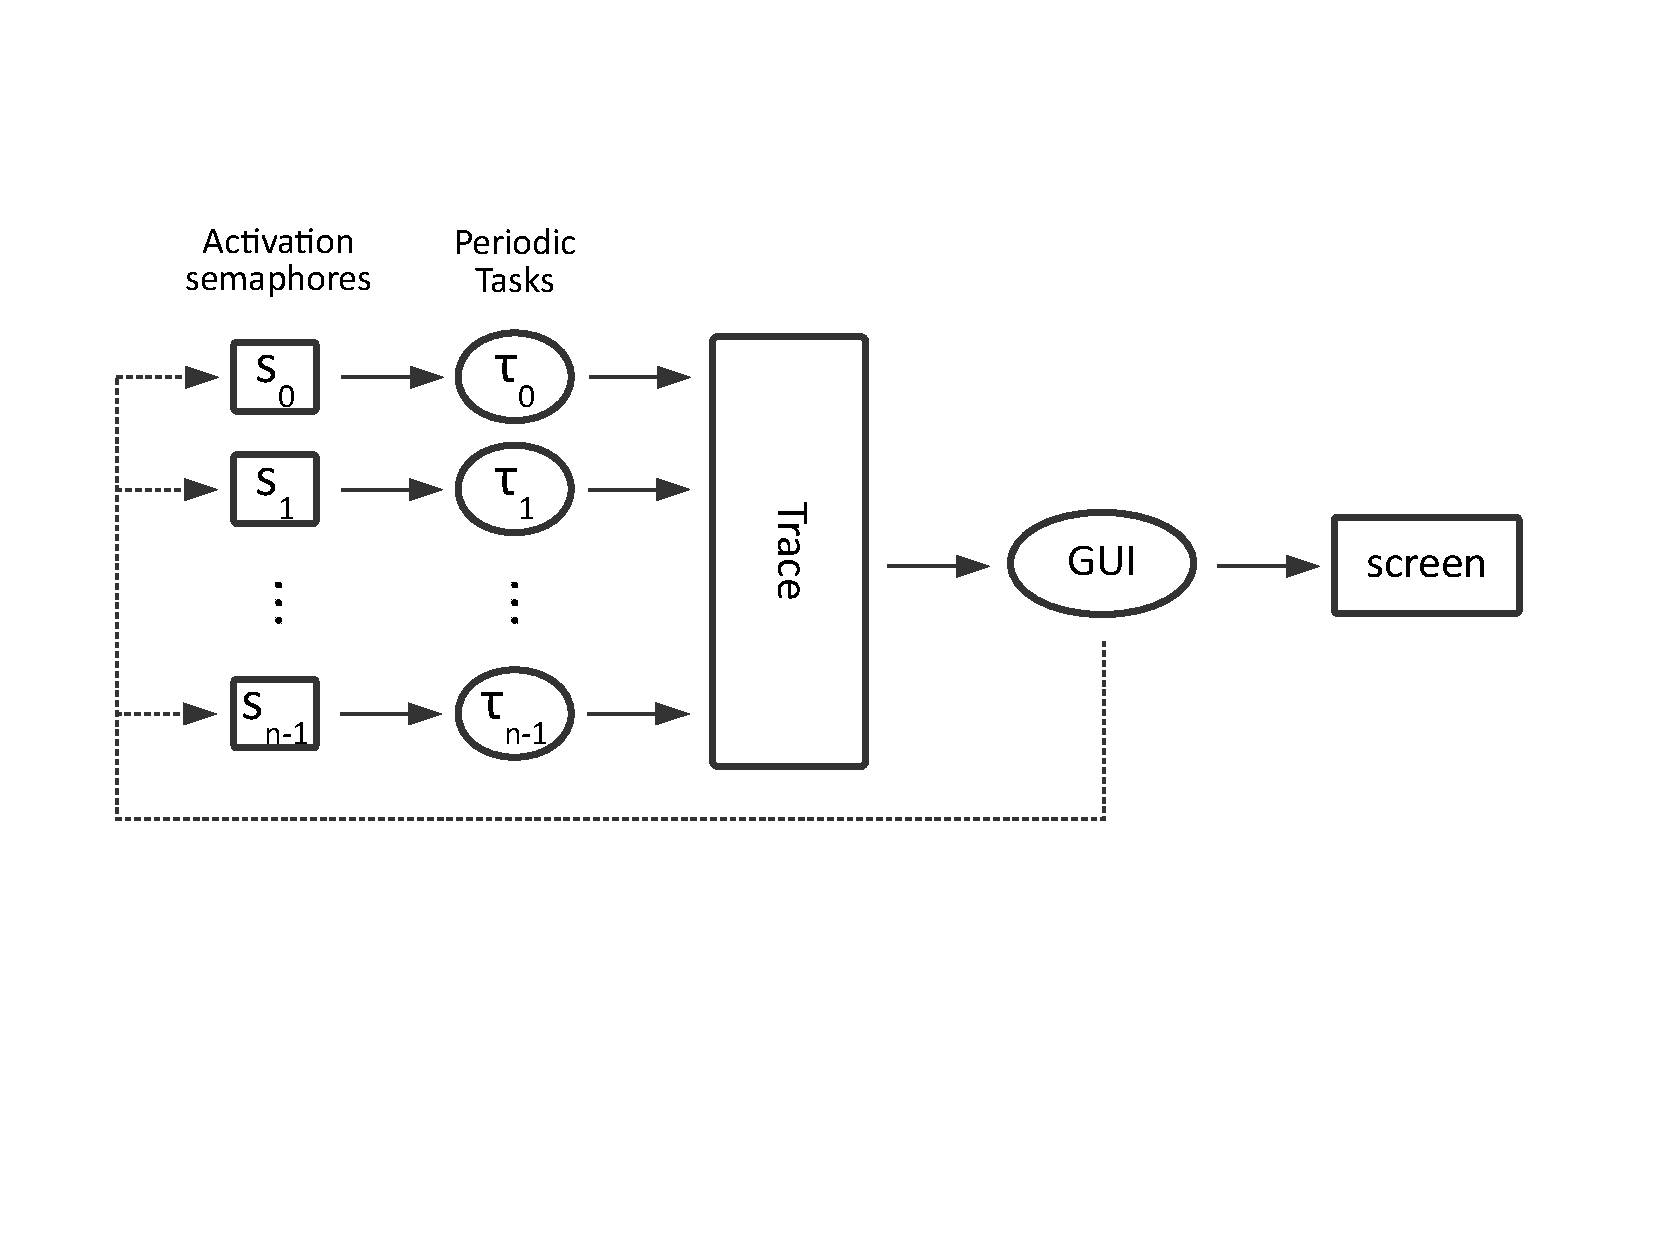
\includegraphics[width=.9\textwidth,trim=0cm 7cm 0cm 3.5cm,clip]{img/tasks_resources_diagram.pdf}
  \caption{\label{fig:architecture} A representation of the interactions among the spawned threads. Note that, other than the ones here represented, the periodic tasks themselves may have extra dependencies and interactions, according to the provided description file.}
\end{figure}

Figure~\ref{fig:architecture} represents the spawned threads and their dependencies, excluding the interactions required by the shared resources specified in the given task set file. Also note that while the tasks do synchronize for writing to the shared trace, the reading thread does not require mutual exclusion.

\subsection{Tasks and tracing}\label{sec:tasks}
In order to track the execution of the tasks in user space, tasks share a global tick counter (the \mono{tick} field in \mono{struct taskset}).
Thus, each task operation consists of an atomic increment to the tick counter, after having checked whether the private counter is up-to-date with the global one: if this is not the case, a context switch is detected and saved into the global \mono{struct trace} instance.

Because these operations are required to be executed atomically, the tasks synchronize using a binary semaphore (the \mono{task\_lock} field in \mono{struct taskset}).
This set-up causes the tasks to behave approximately as if they were running on a single-processor machine, where the global tick counter emulates the processor's clock.


\subsubsection{Task scheduling and priorities}\label{sec:tasks:prio}
All threads that are associated to tasks are instructed to be scheduled with the so-called ``real-time'' scheduling algorithm \mono{SCHED\_RR}\cite{man-sched}, and they are assigned a fixed priority as specified in the task set definition file. This way, the threads scheduling is left to the kernel, while the program simply observes and tracks its behaviour as described above.


\subsubsection{Tracking idle time}\label{sec:tasks:idle}
In order to also track idle time, an extra simplified ``idle'' task is run together with every task set. Its body consists of busily acquiring the global lock and incrementing the tick, while running with a priority that is lower than any other thread. This way, even when no other thread is running, the trace is kept up-to-date.

In order to prevent the idle thread to consume an excessive amount of resources, it is possible to force it to sleep briefly at every iteration using the \mono{-{}-idle-sleep} flag. This is especially useful if the user wants to observe the console output while the task set is running: apparently, a busily-running thread prevents the console output to be flushed properly; however, because this appeared to have an impact on the task scheduling, it is turned off by default. The same result was pursued by issuing a call to \mono{pthread\_yield()} (which can be enabled with \mono{-{}-idle-yield}), but it turned out to have no visible effect.

Note that, in some cases, the idle thread may be executed for a few iterations even if a higher-priority task is ready: this is probably to be imputed to the semaphore behaviour described in section~\ref{sec:tasks:affinity}.

\subsubsection{Shared resources}\label{sec:tasks:resources}
Emulated shared resources are handled with the use of POSIX mutex: each task section can operate on one resource (or on the special ``no resource'' \mono{R0}).
The user can select the protocol to be used for priority-inversion avoidance through the \mono{-p PROTO} or \mono{-{}-protocol=PROTO}, which shall be among \mono{NONE} for no protocol, \mono{INHERIT} for priority inheritance or \mono{PROTECT} for priority ceiling: this is mapped directly on the type of mutex that is initialized, as described in the corresponding POSIX man-page\cite{man-mutexproto}.

Note that when using priority ceiling (\mono{PROTECT}), there is no need to manually specify the ceiling, as it will be automatically inferred from the tasks' definitions. When running with the default output verbosity, the program will report to the console the priority ceiling for each resource.

\subsubsection{CPU load}\label{sec:tasks:cpuload}
Together with the schedule, the CPI load is plotted on the graphical interface. Note that, because the tasks duration is measured in ``number of operations'', the program does not have the notion of the remaining computation time for the tasks, so it can't compute the \textit{instantaneous load} as defined by Buttazzo and Stankovic\cite{BS-instantaneous-load}.

Instead, the displayed load is computed a posteriori by simply measuring the
$\frac{\text{non-idle time}}{\text{time interval}}$
ratio in a given sliding window. For this reason, the load can only be computed after a whole time window has passed since the tasks activation.
Note that, given this definition, the measured load is always in the $[0,1]$ interval: an overload condition is thus indicated by a load of $1$ lasting for a sustained period.

\subsubsection{CPU Affinity setting}\label{sec:tasks:affinity}
Note that, even if the global \mono{task\_lock} semaphore should be enough to guarantee that the tasks behave as if they were on a single-processor machine, this results in an enormous number of context switches, which in turn cause the trace space to be filled quickly and the GUI to have problems in displaying it.
My best guess is that this happens because threads are allowed to run on different processors while outside their critical sections, quickly reaching their next call to \mono{sem\_wait}, causing the kernel to preempt the running thread after a ridiculous amount of steps (3--20 in some trials) in the effort to guarantee non-starvation of waiting threads. To prevent this, by default, task threads are forced to run on the same processor (chosen at start-up time) using the affinity mechanism\cite{man-pthread-affinity}\cite{man-affinity}.
To restore the old behaviour and see what it looks like, use the \mono{-{}-no-affinity} flag (when doing this, I advise opening another shell and preparing to issue \mono{killall -9 scheduletrace}).


\subsection{Graphical User Interface}\label{sec:gui}
The program's GUI is implemented using the Allegro graphics library\footnote{Allegro -- A game programming library: \mono{http://alleg.sourceforge.net} .}.
All the GUI-related work is performed by a dedicated periodic thread which, with a 60 Hz frame rate, refreshes the plotting area on the screen reading the execution information from the shared \mono{struct trace} instance and according to the current visualization settings (scale and offset) required by the user.

In order to reduce the possible interference of the GUI thread on the tasks scheduling, this operation was chosen not to be semaphore-protected. This is the main reason why the trace is implemented as an ever-growing buffer, rather than a circular buffer or a linked-list: this way, the GUI can safely read all the recorded events up to the current length without the possibility for the tasks to write over past events. Note this also implies that once the trace gets full, new events are discarded.


\section{Sample runs}\label{sec:runs}

\begin{figure}
  \centering
  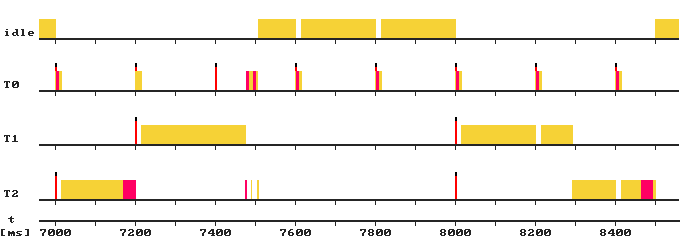
\includegraphics[width=1\textwidth]{img/inversion.png}
  \caption{\label{fig:inversion} The scheduling trace during a priority-inversion phenomenon: at 7200 ms, task \mono{T2} is running a critical section and is preempted by \mono{T0}. However, when \mono{T0} tries to enter its own C.S. it can't, and it must wait until \mono{T1} has completed for \mono{T3} to end its own C.S. and finally be allowed to run, after missing its deadline at 7400 ms. Note that colors have been modified for printing friendliness.}
\end{figure}

The application comes with some sample task set files in the \mono{tasksets} folder. Note that, because the task sections lengths are specified with their operations count, it is possible that on other machines (or changing the external workload) their behaviour differ from the intended one. For the same reason, it is advisable to set a static CPU frequency during the tests, so as to increase uniformity across consecutive runs.

\begin{figure}
  \centering
  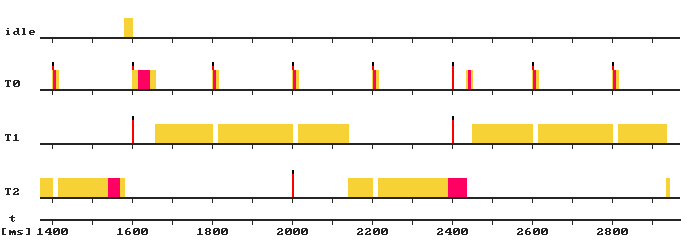
\includegraphics[width=1\textwidth]{img/noinversion_ceiling.png}
  \caption{\label{fig:noinversion-ceiling} The scheduling trace in a situation similar to the one in figure~\ref{fig:inversion}, but with the priority ceiling protocol enabled: at 2400 ms, \mono{T0} and \mono{T1} are activated while \mono{T2} is in its C.S, but this time, because \mono{T2} is owning the resource, it keeps executing until the end of its C.S., then \mono{T0} and \mono{T1} can run without blocking and finally \mono{T2} completes its execution.}
\end{figure}

Figure~\ref{fig:inversion} shows an example of running \mono{scheduletrace} with \mono{-f tasksets/inversion} and \mono{-p none} (so that no priority-inversion avoidance protocol will be in use), while figures \ref{fig:noinversion-ceiling} and \ref{fig:noinversion-inherit} show a similar situation using, respectively, \mono{-p protect} and \mono{-p inherit}, highlighting the different behaviours of the resource sharing protocols. The \mono{inversion} task set is designed to cause priority-inversion, with the high-rate task \mono{T0} sharing a resource with the low-rate \mono{T2}: while the length of the critical section of \mono{T2} is comparable to the run-time of \mono{T0}, in case of priority-inversion the mid-rate task \mono{T1} can get to execute before \mono{T0}, causing it to miss its deadline.

\begin{figure}
  \centering
  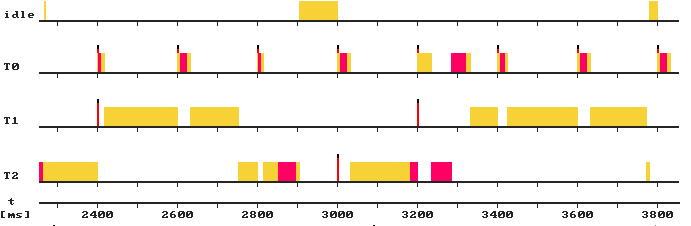
\includegraphics[width=1\textwidth]{img/noinversion_inherit.png}
  \caption{\label{fig:noinversion-inherit} The scheduling trace in a situation similar to the one in figure~\ref{fig:inversion}, but with the priority inheritance protocol enabled: at 3200 ms, \mono{T0} and \mono{T1} are activated while \mono{T2} is in its C.S, but when \mono{T0} requests to enter the C.S. \mono{T2} inherits its priority, allowing it to release the resource and let \mono{T1} complete on time.}
\end{figure}


\section{Conclusions and limitations}
\mono{scheduletrace} is a useful tool for graphically displaying what is going on with the scheduling of periodic tasks, which may find applications for didactic purposes or, in the most rosy case, to ease the development of scheduling algorithms.

It has, however a number of limitations and some missing features that may ease its usage. As discussed in section~\ref{sec:runs}, it is quite a pain to produce reproducible behaviours when defining a task set; while this is intrinsic into the scheduling problem in general, sharing with other a critical run could be eased by allowing to load and browse the trace produced by a previous run. Other interesting extensions could be to provide the capability of asynchronously activate the tasks, or to include different types of aperiodic servers and the possibility to specify and activate aperiodic jobs.

As discussed in section~\ref{sec:tasks:cpuload}, the tool currently does not support estimating computation times. In principle, it could be achievable to estimate at run-time the computing times and thus be able to compute and plot the instantaneous load deadlines and remaining computation time into account, while adaptively correcting the speed estimate for the CPU as perceived by the running program. However, this would require adding non-negligible complexity to the program. A simpler approach would be to report the average computation speed to the user and allow them to run the next instance using that estimate.

Further smaller improvements that could increase the usefulness and usability of this tool are detailed in the README file.


\section*{Further documentation}
\addcontentsline{toc}{section}{Further documentation}
\label{sec:docs}

Further bits of information about \mono{scheduletrace} can be found bundled with its source code:

\begin{itemize}
\item For the building instructions, refer to \mono{README.md} file in the project tree root. Spoiler: put yourself in the project root and run \mono{scons} or, if missing, \mono{make}.
\item For a detailed list of command line options, compile and run with the \mono{-h} or \mono{-{}-help} flag.
\item The taskset file format is also described in the \mono{README.md} file.
\item A list of interactive commands is available directly on-screen, when \mono{-{}-no-gui} is \textit{not} specified.
\end{itemize}

% example with minipage
\begin{comment}
\begin{figure}
  \begin{minipage}[b]{.5\linewidth}
    \includegraphics[width=1.0\linewidth,trim=2cm 1cm 1.5cm 1cm,clip]{images/delivery_9-Y.png}
    \subcaption{\label{fig:delivery:a}Node 9 sending to the yellow group.}
  \end{minipage}%
  \begin{minipage}[b]{.5\linewidth}
    \includegraphics[width=1.0\linewidth,trim=2cm 1cm 1.5cm 1cm,clip]{images/delivery_3-R.png}
    \subcaption{\label{fig:delivery:b}Node 3 sending to the red group.}
  \end{minipage}
  \caption{\label{fig:delivery}Color-scale representation of the delivery ratio at the target nodes.}
\end{figure}
\end{comment}


\begin{thebibliography}{99}
% \addcontentsline{toc}{section}{References}  % made redundant by tocbibind

\bibitem{man-sched}
  VV.AA.
  \textit{SCHED(7)}.
  Linux Programmer's Manual.
  Linux man-pages.
  2014.
  %\\
  %\texttt{https://web.archive.org/web/20141101222734/\\
  %  http://man7.org/linux/man-pages/man7/sched.7.html}

\bibitem{man-mutexproto}
  VV.AA.
  \textit{PTHREAD\_MUTEXATTR\_GETPROTOCOL(3P)}.
  POSIX Programmer's Manual,
  IEEE/The Open Group.
  2013.

\bibitem{man-pthread-affinity}
  VV.AA.
  \textit{PTHREAD\_SETAFFINITY\_NP(3)}.
  Linux Programmer's Manual.
  Linux man-pages.
  2014.

\bibitem{man-affinity}
  VV.AA.
  \textit{SCHED\_SETAFFINITY(2)}.
  Linux Programmer's Manual.
  Linux man-pages.
  2014.

\bibitem{BS-instantaneous-load}
  G. C. Buttazzo, J. Stankovic.
  \textit{Adding robustness in dynamic preemptive scheduling}.
  In D. S. Fussel and M. Malek, editors, Responsive Computer Systems: Steps Toward Fault-Tolerant Real-Time Systems.
  Kluwer Academic Publishers.
  1995.

\end{thebibliography}


% \section{Heading on level 1 (section)}
% \begin{align}
%     \begin{split}
%     (x+y)^3     &= (x+y)^2(x+y)\\
%                     &=(x^2+2xy+y^2)(x+y)\\
%                     &=(x^3+2x^2y+xy^2) + (x^2y+2xy^2+y^3)\\
%                     &=x^3+3x^2y+3xy^2+y^3
%     \end{split}
% \end{align}

% \subsection{Heading on level 2 (subsection)}
% \begin{align}
%     A =
%     \begin{bmatrix}
%     A_{11} & A_{21} \\
%     A_{21} & A_{22}
%     \end{bmatrix}
% \end{align}

% \subsubsection{Heading on level 3 (subsubsection)}

% \paragraph{Heading on level 4 (paragraph)}


% \section{Lists}

% \subsection{Example for list (3*itemize)}
% \begin{itemize}
%     \item First item in a list
%         \begin{itemize}
%         \item First item in a list
%             \begin{itemize}
%             \item First item in a list
%             \item Second item in a list
%             \end{itemize}
%         \item Second item in a list
%         \end{itemize}
%     \item Second item in a list
% \end{itemize}

% \subsection{Example for list (enumerate)}
% \begin{enumerate}
%     \item First item in a list
%     \item Second item in a list
%     \item Third item in a list
% \end{enumerate}

%%% End document
\end{document}